\documentclass[tikz,border=10pt,12pt]{standalone}
% Shared preamble for standalone-compiled dc_paper figures.
% Copies just the bits of dc_paper.tex's preamble that figures need.

\usepackage{amsmath,amssymb,amsthm,mathtools,bm}
\usepackage{siunitx}
\sisetup{detect-all,group-separator={,},per-mode=symbol}

\usepackage[T1]{fontenc}
\usepackage{xcolor}
\usepackage{enumitem}
\usepackage{mathpazo}                % Palatino body + matching math
\usepackage[scaled=0.92]{helvet}     % Helvetica sans
\usepackage{courier}                 % monospace
\usepackage{microtype}

% --- IA brand colour palette (must match dc_paper.tex) ---
\definecolor{iadark}{HTML}{1B1815}
\definecolor{iabone}{HTML}{FAFAF7}
\definecolor{iaaccent}{HTML}{A04A1F}
\definecolor{iataupe}{HTML}{F2EDE6}
\definecolor{iarule}{HTML}{3A332D}
\definecolor{iagrey}{HTML}{5A524A}

% --- graphics ---
\usepackage{tikz}
\usepackage{circuitikz}
\usepackage{pgfplots}
\pgfplotsset{compat=1.18}
\usetikzlibrary{arrows.meta,positioning,shapes.geometric,calc,fit,
                decorations.pathreplacing,decorations.markings,
                shadows.blur,backgrounds}

% --- math macros from dc_paper.tex preamble (figures use them) ---
\newcommand{\E}{\mathbb{E}}
\newcommand{\Var}{\operatorname{Var}}
\newcommand{\Cov}{\operatorname{Cov}}
\newcommand{\Cor}{\operatorname{Cor}}
\newcommand{\Prb}{\mathbb{P}}
\newcommand{\R}{\mathbb{R}}
\newcommand{\N}{\mathbb{N}}
\newcommand{\1}{\mathbf{1}}
\newcommand{\VaR}{\operatorname{VaR}}
\newcommand{\TVaR}{\operatorname{TVaR}}
\newcommand{\ES}{\operatorname{ES}}
\newcommand{\dd}{\mathrm{d}}
\newcommand{\given}{\,\vert\,}
\newcommand{\set}[1]{\left\{#1\right\}}
\newcommand{\norm}[1]{\left\Vert #1 \right\Vert}
\DeclareMathOperator*{\argmin}{arg\,min}
\DeclareMathOperator*{\argmax}{arg\,max}

% \textwidth has no meaning in standalone class; give it a value matching
% the paper's A4 + 1-inch margins so any leftover \resizebox{\textwidth}
% gracefully sizes the figure to that nominal width.
\setlength{\textwidth}{15.92cm}

\begin{document}
\pagecolor{iabone}
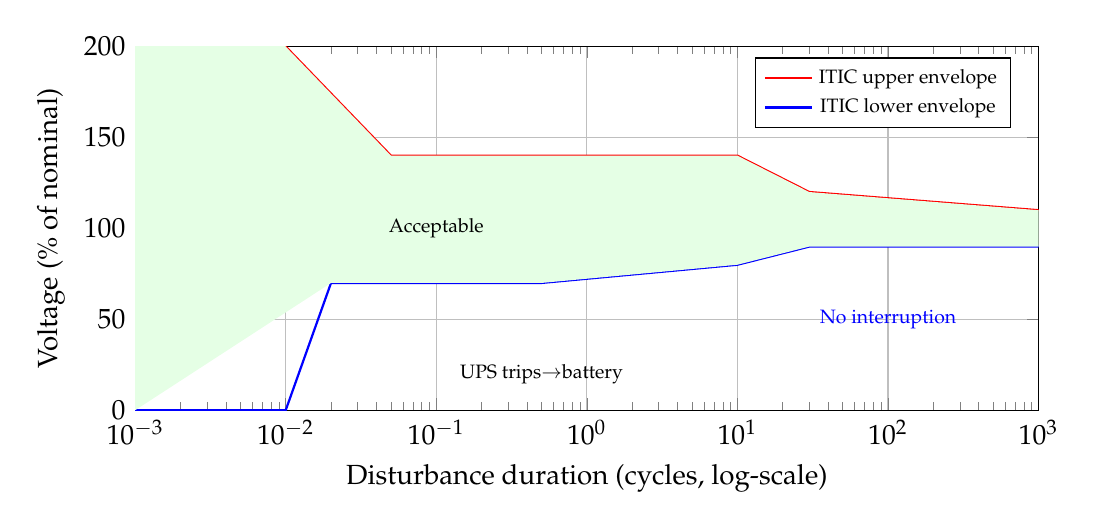
\begin{tikzpicture}
\begin{semilogxaxis}[
  width=0.82\linewidth, height=6.2cm,
  xlabel={Disturbance duration (cycles, log-scale)},
  ylabel={Voltage (\%\ of nominal)},
  xmin=0.001, xmax=1000, ymin=0, ymax=200,
  grid=major,
  legend pos=north east,
  legend style={font=\scriptsize},
  log basis x=10,
]
% Upper envelope (overvoltage tolerance)
\addplot[red,thick] coordinates {
  (0.001,500) (0.01,200) (0.05,140) (0.5,140)
  (10,140) (30,120) (1000,110) };
\addlegendentry{ITIC upper envelope}

% Lower envelope (undervoltage tolerance)
\addplot[blue,thick] coordinates {
  (0.001,0) (0.01,0) (0.02,70) (0.5,70)
  (10,80)  (30,90)  (1000,90) };
\addlegendentry{ITIC lower envelope}

% Acceptable region shading
\addplot[fill=green!10,draw=none,forget plot] coordinates
  { (0.02,70) (0.5,70) (10,80) (30,90) (1000,90) (1000,110)
    (30,120) (10,140) (0.5,140) (0.05,140) (0.01,200) (0.001,500)
    (0.001,0) (0.02,70) };

% Annotations
\node[font=\scriptsize] at (axis cs:0.1,100) {Acceptable};
\node[font=\scriptsize,red] at (axis cs:0.005,300) {No damage};
\node[font=\scriptsize,blue] at (axis cs:100,50) {No interruption};
\node[font=\scriptsize] at (axis cs:0.5,20)  {UPS trips$\to$battery};
\end{semilogxaxis}
\end{tikzpicture}
\end{document}
